% Glava dokumenta
\documentclass[slovene]{beamer}
\usepackage[utf8x]{inputenc}
\usepackage{lmodern}
\usepackage[T1]{fontenc}
\usetheme{Antibes} % izbira nastavitev oblike in barv strani
%\usecolortheme{beetle}
\usepackage{tikz}
\usepackage[slovene]{babel}
%\usetikzlibrary{arrows}
\usepgflibrary{arrows}% for more options on arrows
\usetikzlibrary{arrows.meta}
\usetikzlibrary{positioning}
\usepackage{varwidth}
\usepackage{color}
\usepackage{amsmath} 

\uselanguage{slovene}
\languagepath{slovene}
\deftranslation[to=slovene]{Definition}{Definicija}
\usepackage{outlines}

\usepackage[customcolors,norndcorners]{hf-tikz}
\usetikzlibrary{calc} %% added

\graphicspath{{./slike/}{./slike/fazni_diagrami/}{../eps_pdf/}}
\DeclareGraphicsExtensions{.eps,.jpeg,.png,.gif,.pdf}
\usepackage[outdir=../uporabljene_slike/]{epstopdf}
\epstopdfsetup{
	suffix=,
}

\newcommand{\Alpha}{A}
\newcommand{\Beta}{B}
\newcommand{\Epsilon}{E}
\newcommand{\Kappa}{K}
\newcommand{\dif}{\mathrm{d}}

\setbeamertemplate{navigation symbols}{}
\setbeamertemplate{section in toc}[sections numbered]
\setbeamertemplate{subsection in toc}[subsections numbered]

\setlength{\abovedisplayskip}{0pt}
\setlength{\belowdisplayskip}{0pt}

%  15 slajdov:
%  1-4 uvod: vesikli, ograjeni vesikli, mitohondrij
%  a. vesikli na splosno
%  b. mitohondriji kot motivacija
%  c. ograjeni vesikli: pregled rezultatov
%  d. Bor: tesna ograditev
%  5 namen dela
%  6 metodologija: upogibna elasticnost, ADE teorija, medmembranska interakcija
%  7 metodologija: robovi itd. eksperimentalni rezultati za mitohondrij?
%  8-9 modelske oblike
%  10-13 rezultati
%  14 interpretacija: prehod med kondenziranim in ortodoksnim stanjem
%  15 zakljucek: mozne razsiritve, gibek zunanji vesikel

\title{Lipidni vesikli v valjasti ograditvi}

\author[Jure Lapajne]{Jure Lapajne\\{\small Mentor: prof. dr. Primož Ziherl}}

\date{6.9.2018}


\begin{document}
	
	\frame{\titlepage}
	\setlength{\abovedisplayskip}{3pt}
	\setlength{\belowdisplayskip}{3pt}


	
\section{Lipidni vesikli}
%\{Nastanek}

\begin{frame}
	\frametitle{Lipidni vesikli}
	\begin{minipage}[]{0.17\linewidth}
		amfifilna molekula
	\end{minipage}%
	\begin{minipage}{0.12\linewidth}
		
\begin{tikzpicture}
		\draw [blue, ->,  -stealth , ultra thick   ] (0 , 0) -- (1,0);
		\end{tikzpicture}
	\end{minipage}%
	\begin{minipage}[]{0.35\linewidth}
		\centering
		fosfolipidni dvosloj
	\end{minipage}
	\begin{minipage}{0.12\linewidth}
		
\begin{tikzpicture}
		\draw [blue, ->,  -stealth , ultra thick, align=center] (0 , 0) -- (1,0) ;
		\end{tikzpicture}
	\end{minipage}%
	\begin{minipage}[]{0.2\linewidth}
		lipidni vesikel	
	\end{minipage}
	\\
	\vspace{0.2cm}
	
	\begin{minipage}[]{0.17\linewidth}
		\centering
		\includegraphics[width=1.6cm]{palmitat.png}
	\end{minipage}%
	\begin{minipage}{0.12\linewidth}
		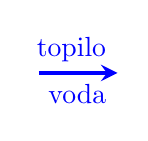
\begin{tikzpicture}
		\draw [blue, ->,  -stealth , ultra thick   ] (0 , 0) -- (1,0) node[anchor=south east] {topilo} node[anchor=north east, align=center] {voda};
		\end{tikzpicture}
	\end{minipage}%
	\begin{minipage}[]{0.35\linewidth}
		\centering
		\includegraphics[width=4cm]{bilayer_prevedeno.png}	
	\end{minipage}
	\begin{minipage}{0.12\linewidth}
		
\begin{tikzpicture}
		\draw [blue, ->,  -stealth , ultra thick   ] (0 , 0) -- (1,0) ;
		\end{tikzpicture}
	\end{minipage}%
	\begin{minipage}[]{0.2\linewidth}
		\centering
		\includegraphics[width=3cm]{vesicle_membrane.jpg}
	\end{minipage}
	\\
	\vspace{0.2cm}
	\begin{minipage}[]{\linewidth}
		membrane celic in celičnih organelov:
		\begin{outline}[itemize] 
			\1 sestava: fosfolipidni dvosloj, proteini
			\1 velik nabor oblik: citoskelet, kemijska sestava membrane in vsebina celice/organela 
	\end{outline}
		\end{minipage}
	
		\begin{tikzpicture}[remember picture,overlay]
	\node (vir2) at ($(current page.center)+ (-1.1cm,-0.9cm)$) {{\fontsize{3}{4}\selectfont  R. F. Boyer, 2005}};
	
	\node[rotate = 90] (vir1) at ($(current page.center)+ (-5.45cm,-1cm)$) {{\fontsize{3}{4}\selectfont  G. Cooper in R. Hausman, 2005}};
	
	\node[rotate = 0] (vir2) at ($(current page.center)+ (5.3cm,-1.8cm)$) {{\fontsize{3}{4}\selectfont  https://www.moltemplate.org/}};
	\end{tikzpicture}
	
\end{frame}


%\subsection{mitohondrij}
\begin{frame}
	\frametitle{Mitohondrij}
	\begin{minipage}[]{0.5\linewidth}
		\begin{outline}[itemize]
			\1 dve membrani:\\notranja in zunanja
			\1 podolgovata oblika,\\številni uvihki
			\1 dve stanji mitohondrija:
			 \2 ortodoksno:  intenzivno celično dihanje,\\tubularni uvihki
			 \2 kondenzirano: počasno celično dihanje,\\lamelarni uvihki
			\1 notranja membrana tvori gube - posledica prostorske ograditve?
		\end{outline}	
	\end{minipage}%
	\begin{minipage}[]{0.5\linewidth}
	  \begin{minipage}[]{0.5\linewidth}
	  	\centering
		\includegraphics[scale=0.45]{mitochondrion_electron_microcope.jpg}
	  \end{minipage}
	  \vspace{0.5cm}
	  \\
      \begin{minipage}[]{\linewidth}
      	\centering
	    \includegraphics[scale=0.13]{{3d_tomogram}.png}
	  \end{minipage}
    \end{minipage}

		\begin{tikzpicture}[remember picture,overlay]
		\node (vir2) at ($(current page.center)+ (3.8cm,-0.6cm)$) {{\fontsize{3}{4}\selectfont  J. Nishiura}};
		\node[rotate = 0] (vir1) at ($(current page.center)+ (5.2cm,-4.1cm)$) {{\fontsize{3}{4}\selectfont T. G. Frey et al., 2002}};
		\end{tikzpicture}
\end{frame}

\begin{frame}
	\frametitle{Ograjeni vesikli}
	\begin{minipage}[]{0.5\linewidth}
		\begin{itemize}
			\item površina vesikla večja od površine ograditve
			\item najpreprostejša ograditev: sfera
			\item dobro ujemanje med eksperimentalnimi opazovanji ter numeričnimi in analitičnimi izračuni na osnovi teorije elastičnosti
		\end{itemize}	
	\end{minipage}%
	\begin{minipage}{0.5\linewidth}
		\includegraphics[scale=0.2]{ograjeni_vezikli_primer3.png}
	\end{minipage}
		\begin{tikzpicture}[remember picture,overlay]
		\node[rotate = 90] (vir2) at ($(current page.center)+ (4.65cm,-2.60cm)$) {{\fontsize{3}{4}\selectfont  A. Sakashita et al., 2014}};
		\end{tikzpicture}
\end{frame}

\begin{frame}
	\frametitle{Preprost fizikalni model (Kavčič 2014)}
	\begin{minipage}[]{0.5\linewidth}
		motivacija:
	\begin{itemize}
		\item enostaven izračun energije, površine, prostornine...
		\item analitični izrazi razkrijejo bistvene odvisnosti
	\end{itemize}
	značilnosti:
		\begin{itemize}
			\item geometrijsko preproste oblike: sfere, sferne kapice, valjasti odseki...
			\item tesna ograditev
		\end{itemize}	
	\end{minipage}%
	\begin{minipage}{0.5\linewidth}
		\includegraphics[scale=0.2]{bor_rezultati.png}
	\end{minipage}
		\begin{block}{namen dela}
			razširitev modela na vesikle v valjasti ograditvi
		\end{block}
		\begin{tikzpicture}[remember picture,overlay]
		\node[rotate = 90] (vir2) at ($(current page.center)+ (6.05cm,-1cm)$) {{\fontsize{3}{4}\selectfont B. Kavčič, 2014}};
		\end{tikzpicture}
\end{frame}


\section{Fizikalni opis vesiklov}
	\begin{frame}
		\frametitle{Parametri za opis vesiklov}
		parametre definiramo relativno glede na sfero z enako površino kot vesikel
		\begin{minipage}{0.5\textwidth}
	   		\begin{block}{polmer sfere}
	   			\vspace*{-\baselineskip}\setlength\belowdisplayshortskip{0pt}
	   			\begin{equation}
	   			R_s=\sqrt{\frac{A}{4\pi}} = 1 \nonumber
	   			\end{equation}
	   		\end{block}
   		\begin{block}{reducirana prostornina}
   			\vspace*{-\baselineskip}\setlength\belowdisplayshortskip{0pt}
   			\begin{equation}
   			v=V_{}/(4\pi R_s^3/3) \nonumber
   			\end{equation}
   		\end{block}
		\end{minipage}%
		\begin{minipage}{0.5\textwidth}
			\hspace{0.5cm}
				\includegraphics[scale=0.2]{zeks_svetina_da_veziklov.png}
		\end{minipage}	
	\begin{minipage}{1\textwidth}
		\begin{block}{reducirana razlika površin monoslojev}
			\vspace*{-0.9\baselineskip}\setlength\belowdisplayshortskip{0pt}
			\begin{equation}
			\Delta a=\frac{1}{8\pi R_s}\int H \dif A \nonumber
			\end{equation}
		\end{block}
	\end{minipage}
		\begin{tikzpicture}[remember picture,overlay]
		\node[rotate = 90] (vir2) at ($(current page.center)+ (4.8cm,-1.0cm)$) {{\fontsize{3}{4}\selectfont S. Svetina in B. Žekš, 2002}};
		\end{tikzpicture}	
	\end{frame}
		
		
     \begin{frame}
     	\frametitle{Brezdimenzijska energija vesikla}
     	\begin{minipage}{0.7\textwidth}
     	\begin{itemize}
     		\itemsep 0em 
     		\item lokalna upogibna energija
     		\begin{equation} \label{eq:lokalni_prispevek}
     		w_b=\frac{1}{16\pi}\int (2H)^2\dif A,
     		\nonumber
     		\end{equation}
     		pri čemer je H povprečna ukrivljenost
     		\begin{equation}
     		H=\frac{1}{2}\left( 1/R_1 + 1/R_2 \right) 
     		\nonumber
     		\end{equation}
     			\item medmembranska interakcija
     			\begin{equation}
     			w_a=-\gamma\int_{\substack{ \text{stične ploskve}}} \frac{\dif A}{4\pi R_s^2} \nonumber
     			\end{equation}
     			$\gamma$: moč medmembranske interakcije
     		\end{itemize}
     	\end{minipage}%
     	\begin{minipage}{0.3\textwidth}
     		\hspace{1cm}
     		\includegraphics[scale=0.3]{povprecna_ukrivljenost.pdf}
     	\end{minipage}	
     	\begin{itemize}	
     		\item nelokalna upogibna energija oziroma \emph{Area Difference Elasticity} (ADE) člen
     		\begin{equation} \label{ade_energija}
     		w_r=q(\Delta a-\Delta a_0)^2 \nonumber
     		\end{equation}
     		$q$: razmerje med nelokalno in lokalno upogibno konstanto
     	\end{itemize}
     		\begin{tikzpicture}[remember picture,overlay]
			 \node[rotate = 00] (vir2) at ($(current page.center)+ (5.5cm,-0.8cm)$) {{\fontsize{3}{4}\selectfont      U. Seifert, 2004}};
			 \end{tikzpicture}
     \end{frame}
     
     

\section{Model}
\subsection{Oblike}
	\begin{frame}
		\frametitle{Ograditev in modelske oblike}
		\begin{tikzpicture}[remember picture,overlay]
		\node (ograditev) at ($(current page.north west)+ (2.5cm,-4.9cm)$)
		{\includegraphics[width=.27\textwidth]{ograditev.pdf}} node[align=center, above, yshift=1.6cm, xshift=1.2cm] (Vograditev) {valjasta ograditev\\brez končnih ploskev};
		
		\node[] (vesikel) at ($(ograditev.east) + (2.2, 0)$)
		{\includegraphics[width=.27\textwidth]{vesikel.pdf}} node[align=center, xshift=4.5cm] at (Vograditev) {zunanja oblika vesikla};
		
		\node[align=center] at ($(vesikel.south)+(2.5, -0.7)$) {polnilno razmerje: $\eta=V / LR^2$\\$V$: volumen vesikla};
		
		\node (presek) at ($(ograditev.east) + (6.2, 0)$)
		{\includegraphics[width=.3\textwidth]{presek_vesikla.pdf}} node[align=center, xshift=8.2cm] at (Vograditev) {presek vesikla};
		
		\node (uvihek) at ($(current page.south) + (-4,1.8)$) {\includegraphics[width=.22\textwidth]{StenaRob.png}} ;
		
		\node[above, yshift=1cm] at (uvihek) {membranski uvihek};
		
		\def \dx {-0.2cm}
		\def \dy {-0.65cm}
		\def \Sdim {0.1cm}
		\definecolor{FillColor1}{RGB}{102,178,255};
		\def \gap {0.4cm}
		
		\draw [fill=red, red] ($(uvihek.east)+(\dx, \dy)+(0.5*\Sdim, 5*\Sdim)$) circle [radius=(\Sdim)*0.5] node[right, black, align=center, yshift=-0.0cm] {robovi z enotnim polmerom $r$};
		
		\draw [fill=FillColor1, FillColor1] ($(uvihek.east)+(\dx, \dy-\gap)+(0.5*\Sdim, 5*\Sdim)$) circle [radius=(\Sdim)*0.5] node[right, black, align=center] {telo uvihka, odvisno od vrste uvihka};
		\end{tikzpicture}
		
		%\item {  \color{red} robovi z enotnim polmerom $r$}
		%\item {  \color{blue} telo uvihka odvisno od posamezne vrste uvihka}		
	\end{frame}
	
	
	
	\begin{frame}
		\frametitle{Robovi}      
        
    \begin{tikzpicture}[remember picture,overlay]
    \def \center {current page.north}
    \node (box) [xshift=0cm,yshift=-3.5cm] at (\center) {\framebox{\normalsize
       		{\begin{varwidth}{0.7\linewidth}
       			\centering
      			 enoten polmer $r$ vseh robov v vesiklu\\
      			 drugi polmer veliko večji od $r$\\
      			 $H=1/2r$
       			\end{varwidth}}
       	}};
       	
    \draw  [->, thick, blue] (box.south) -- ($ (box.south) + (-4.2,-0.8) $) node[below, black] {trojni rob};
    
    \node[inner sep=0pt] (russell) at (1cm,-1.9cm)
    {\includegraphics[width=.25\textwidth]{bor_slika_3rob_2.png}};
    
    \draw [->, thick, blue]  ($ (box.south) + (-3,-2.8) $) -- ($ (box.south) + (-2,-2.8) $) node[above left, yshift=-0.1cm, xshift=0.05cm, black] {\small{$\alpha=\pi$}};
    
    \draw [->, thick, blue] (box.south) -- ($ (box.south) + (-1.5,-0.8) $) node[below, black] {zunanji rob};
    
    \node[inner sep=0pt] (russell) at (4.2cm,-1.8cm)
    {\includegraphics[width=.22\textwidth]{zunanji_rob_povecanje_povrsine.pdf}};
    
    \draw [->, thick, blue] (box.south) -- ($ (box.south) + (1.5,-0.8) $) node[below, black] {U rob};
    
     \node[inner sep=0pt] (russell) at (7.3cm,-2.5cm)
     {\includegraphics[width=.17\textwidth]{urob_2d.pdf}};
     
 \node[inner sep=0pt] (russell) at (6.5cm,-1.7cm)
 {\includegraphics[width=.17\textwidth]{urob_3d.pdf}};
    
    
    \node[inner sep=0pt] (torus) at (10cm,-1.75cm)
    {\includegraphics[width=.25\textwidth]{torus_uvodni_del_prirejeno.png}};
    
     \node[below, black] at ($ (box.south) + (4.2,-0.8) $) {torusni rob};
     
   	\end{tikzpicture}
		\begin{tikzpicture}[remember picture,overlay]
	\node[rotate = 0] (vir2) at ($(current page.center)+ (-5.1cm,-3.8cm)$) {{\fontsize{3}{4}\selectfont B. Kavčič, 2014}};
	\node[rotate = 0] (vir2) at ($(current page.center)+ (5.1cm,-3.4cm)$) {{\fontsize{3}{4}\selectfont C. Renken et al., 2000}};
	\end{tikzpicture}
	\end{frame}
	
	
	
\begin{frame}
	\frametitle{Modelski vesikli}      		
\begin{tikzpicture}[remember picture,overlay]
\def \center {current page.north}
\node (box) [xshift=0cm,yshift=-3.5cm] at (\center) {\framebox{\normalsize
		{\begin{varwidth}{1.1\linewidth}
			\centering
	membranski uvihek = telo uvihka + skladne oblike robov
			\end{varwidth}}
	}};
	
	\draw  [->, thick, blue] (box.south) -- ($ (box.south) + (-4.5,-0.8) $) node[below, black, align=center] {vesikel s prečno\\steno};
	
	\node[inner sep=0pt] (russell) at (1cm,-1.9cm)
	{\includegraphics[width=.22\textwidth]{vezikel_z_invaginacijo.pdf}};
	
	\draw [->, thick, blue] (box.south) -- ($ (box.south) + (-1.6,-0.8) $) node[below, black, align=center] {vesikel s popolnimi\\prečnimi stenami};
	
	\node[inner sep=0pt] (russell) at (4cm,-1.8cm)
	{\includegraphics[width=.26\textwidth]{delitev_vezikla.pdf}};
	
	\draw [->, thick, blue] (box.south) -- ($ (box.south) + (1.6,-0.8) $) node[below, black, align=center] {vesikel z vzdolžno\\steno};
	
	\node[inner sep=0pt] (russell) at (6.8cm,-1.8cm)
	{\includegraphics[width=.23\textwidth]{vezikel_z_vzdolzno_invaginacijo.pdf}};
	
	
	\draw [->, thick, blue] (box.south) -- ($ (box.south) + (4.5,-0.8) $) node[below, black, align=center] {drevo\\tubulov};
	
	\node[inner sep=0pt] (russell) at (9.9cm,-1.75cm)
	{\includegraphics[width=.27\textwidth]{drevo_slika.pdf}};
	\end{tikzpicture}
\end{frame}

\subsection{Analiza}
\begin{frame}
\frametitle{Upogibna energija in ADE člen modelskih oblik}
	\begin{minipage}{0.5\textwidth}
  		\hspace{0cm}
  		\includegraphics[scale=0.23]{all_vesicle_energy_diagram_R03_eta099.pdf}
	\end{minipage}%
	\begin{minipage}{0.5\textwidth}
		\hspace{0cm}
		\includegraphics[scale=0.18]{ade_model_diskretni_vesikli.pdf}
	\end{minipage}\\
	\vspace{.3cm}
	\begin{minipage}{0.5\textwidth}
		\begin{itemize}
			\item lokalna upogibna energija
			\item $\eta=0.99$, $R=0.3$
			\item vesikel z vzdolžno steno močno izstopa: velika dolžina robov
		\end{itemize}
	\end{minipage}%
	\begin{minipage}{0.5\textwidth}
		\begin{itemize}
			\item diskretna območja stabilnosti posameznih vesiklov
			\item parabole izvirajo iz ADE člena: $q(\Delta a -\Delta a_0)^2$
		\end{itemize}
	\end{minipage}
\end{frame}

\section{Fazni diagrami}
%\subsection{Izraz za minimizacijo}
	\begin{frame}
		\frametitle{Minimizacija energije}
		\begin{block}{energija vesikla}
		\vspace*{-\baselineskip}\setlength\belowdisplayshortskip{0pt}
			\begin{equation}
			w=\underbrace{\frac{1}{16\pi}\int (2H)^2\dif A}_{\substack{\text{lokalna upogibna} \\ \text{energija} }} + \underbrace{ q(\Delta a-\Delta a_0)^2 }_{\substack{\text{nelokalna upogibna} \\ \text{energija}}}-        \underbrace{ \gamma\int_{\substack{ \text{stične ploskve}}} \frac{\dif A}{A} }_{\substack{\text{medmembranska} \\ \text{interakcija}}} 
			\nonumber
			\end{equation}
			$q$: razmerje med nelokalno in lokalno upogibno konstanto\\
			$\gamma$: medmembranska interakcijska konstanta\\
			$\Delta a_0$: ravnovesna vrednost $\Delta a$
		\end{block}
			\begin{itemize}
				\item konstantna površina $A=4\pi$ oziroma $R_s=1$
				\item konstantna reducirana prostornina
				\item konstanten polmer ograditve $R$
				\item polnilno razmerje $\eta$ blizu $1$ 
			\end{itemize}
	\end{frame}
	
	
\subsection{$R=0.3$}

	\begin{frame}
		\frametitle{Fazni diagrami: ni medmembranske interakcije}
		\begin{tikzpicture}[remember picture,overlay]
		\def \xfromcenter  {3.8}
		\def \yfromcenter {0.5}
		
		\node (slika1) at ($(current page.center)+ (-\xfromcenter,\yfromcenter cm)$)
		{\includegraphics[width=.3\textwidth]{{minimizacija_q1_0_q2_0_da0_0_R_0.3_eta_0.995_sirinav_0.002_sirinada_0.05}.pdf}};
		
		\node[anchor=north] at ($(current page.center) + (-0.97*\xfromcenter, \yfromcenter + 1.9)$) {\tiny$R=0.3,  q=0, \gamma=0, \eta=0.995 $};
		
		\node[] (legenda) at ($(current page.center) + (0, \yfromcenter)$)
		{\includegraphics[width=.33\textwidth]{legenda.pdf}} node[align=center, xshift=4.5cm] at (Vograditev) {};
		
		\node (slika2) at ($(current page.center) + (\xfromcenter, \yfromcenter)$)
		{\includegraphics[width=.3\textwidth]{{minimizacija_q1_20*Pi_q2_0_da0_0_R_0.3_eta_0.995_sirinav_0.002_sirinada_0.05}.pdf}};
		
		\node[anchor=north] at ($(current page.center) + (1.03*\xfromcenter, \yfromcenter + 1.9)$) {\tiny$R=0.3,  q=\pi, \gamma=0, \eta=0.995 $};
		
		
	    {
				\setlength{\fboxrule}{0pt}%
		\node[] (itemize1) [below=0cm and 0cm of slika1, xshift=1cm] {\framebox{\normalsize
				{\begin{varwidth}{0.55\linewidth}
					\begin{itemize}
					\item $q=0$: fazni diagram ni odvisen od $\Delta a_0$
					\item $v>0.3$: vesikli s popolnimi in nepopolnimi prečnimi stenami
					\end{itemize}
					\end{varwidth}
					}
			}};
		}
		
	{
	   	\setlength{\fboxrule}{0pt}%
	   	\node (itemize1) [below=0cm of slika2, xshift=-0.4cm] {\framebox{\normalsize
	   			{\begin{varwidth}{0.55\linewidth}
	   				\begin{itemize}
					\item dominira vesikel z vzdolžno steno
					\item $v \approx 0.4$ in $\Delta a_0 \gtrsim 2.5$:\\vesikel s tubuli
	   				\end{itemize}
	   				\end{varwidth}
	   			}
	   		}};
	   	}
		
		\end{tikzpicture}
	\end{frame}
	
	
\begin{frame}
	\frametitle{Fazni diagrami: medmembranski odboj}
	\begin{tikzpicture}[remember picture,overlay]
	\def \xfromcenter  {3.8}
	\def \yfromcenter {0.25}
	
	\node (slika1) at ($(current page.center)+ (-\xfromcenter,\yfromcenter cm)$)
	{\includegraphics[width=.3\textwidth]{{minimizacija_q1_Pi_q2_1250_da0_0_R_0.3_eta_0.995_sirinav_0.002_sirinada_0.05}.pdf}};
	
	\node[anchor=north] at ($(current page.center) + (-0.97*\xfromcenter, \yfromcenter+ 1.9)$) {\tiny$R=0.3,  q=\pi, \gamma=-6000\pi, \eta=0.995 $};
	
	\node[] (legenda) at ($(current page.center) + (0, \yfromcenter)$)
	{\includegraphics[width=.33\textwidth]{legenda.pdf}} node[align=center, xshift=4.5cm] at (Vograditev) {};
	
	\node (slika2) at ($(current page.center) + (\xfromcenter, \yfromcenter)$)
	{\includegraphics[width=.3\textwidth]{{minimizacija_q1_20*Pi_q2_1000_da0_0_R_0.3_eta_0.995_sirinav_0.002_sirinada_0.05}.pdf}};
	
	\node[anchor=north] at ($(current page.center) + (1.03*\xfromcenter, \yfromcenter+1.9)$) {\tiny$R=0.3,  q=20\pi, \gamma=-4000\pi, \eta=0.995 $};
	
	
	{
		\setlength{\fboxrule}{0pt}%
		\node[] (itemize1) [below=0cm and 0cm of slika1, xshift=1cm] {\framebox{\normalsize
				{\begin{varwidth}{0.55\linewidth}
					\begin{itemize}
					\item močna odbojna medmembranska interakcija: območje vesikla s tubuli narašča
					\item $v<0.4$: vesikli z vzdolžnimi stenami
					\end{itemize}
					\end{varwidth}
				}
			}};
		}
		
		{
			\setlength{\fboxrule}{0pt}%
			\node (itemize1) [below=0cm of slika2, xshift=-0.4cm] {\framebox{\normalsize
					{\begin{varwidth}{0.55\linewidth}
						\begin{itemize}
						\item $v\approx0.425$: mehak prehod\\med vesikli z nepopolnimi\\prečnimi stenami 
						\item majhni $v$: vesikel z vzdolžno steno
						\end{itemize}
						\end{varwidth}
					}
				}};
			}
			
			\end{tikzpicture}
		\end{frame}


\subsection{$R=0.5$}

\begin{frame}
	\frametitle{Fazni diagrami: $R=0.5$}
	
	\begin{tikzpicture}[remember picture,overlay]
	\def \xfromcenter  {3.8}
	\def \yfromcenter {-1}
	\def \legendy {0.7 - \yfromcenter}
	\def \legendx {2}
	
\node (legenda1) at ($(current page.center)+ (-\legendx, \legendy)$)
{\includegraphics[width=.3\textwidth]{legenda_del1.pdf}};

\node (legenda2) at ($(current page.center)+ (\legendx, \legendy)$)
{\includegraphics[width=.3\textwidth]{legenda_del2.pdf}};
	
	\node (slika1) at ($(current page.center)+ (-\xfromcenter,\yfromcenter cm)$)
	{\includegraphics[width=.3\textwidth]{{minimizacija_q1_Pi_q2_1500_da0_0_R_0.5_eta_0.98_sirinav_0.01_sirinada_0.05}.pdf}};
	
	\node[anchor=north] at ($(current page.center) + (-0.97*\xfromcenter, \yfromcenter + 2)$) {\tiny$q=\pi, \gamma=-6000\pi, \eta=0.98 $};
	
	\node[] (legenda) at ($(current page.center) + (0, \yfromcenter)$)
	{\includegraphics[width=.3\textwidth]{{minimizacija_q1_Pi_q2_0_da0_0_R_0.5_eta_0.98_sirinav_0.01_sirinada_0.05}.pdf}} node[align=center, xshift=4.5cm] at (Vograditev) {};
	
	\node[anchor=north] at ($(current page.center) + (0.03*\xfromcenter, \yfromcenter + 2)$) {\tiny$q=\pi, \gamma=0, \eta=0.98 $};
	
	\node (slika2) at ($(current page.center) + (\xfromcenter, \yfromcenter)$)
	{\includegraphics[width=.3\textwidth]{{minimizacija_q1_10*Pi_q2_0_da0_0_R_0.5_eta_0.98_sirinav_0.01_sirinada_0.05}.pdf}};
	
	\node[anchor=north] at ($(current page.center) + (1.03*\xfromcenter, \yfromcenter + 2)$) {\tiny$q=10\pi, \gamma=0, \eta=0.98 $};
	
	
	{
		\setlength{\fboxrule}{0pt}%
		\node[] (itemize1) [below=0cm and 0cm of slika1, xshift=1cm] {\framebox{\normalsize
				{\begin{varwidth}{0.55\linewidth}
					\begin{itemize}
					\item močen odboj: območje vesikla s tubuli narašča
					\end{itemize}
					\end{varwidth}
				}
			}};
		}
		{
			\setlength{\fboxrule}{0pt}%
			\node (itemize1) [below=0cm of slika2, xshift=-0.4cm] {\framebox{\normalsize
					{\begin{varwidth}{0.55\linewidth}
						\begin{itemize}
						\item ADE člen: energijsko\\ugodnješi vesikli z delnimi\\prečnimi stenami
						\end{itemize}
						\end{varwidth}
					}
				}};
			}
			
			\end{tikzpicture}

		\end{frame}

	
\subsection{Interpretacija}
	\begin{frame}
	\frametitle{Prevladujoča oblika gub}
\centering{dve stanji mitohondrija glede na prevladujočo obliko gub}
	\vspace{0.2cm}
	\\
	\begin{minipage}[]{0.7\linewidth}
		\centering
		\includegraphics[width=0.9\linewidth]{{orthodox_condensed}.png}
	\end{minipage}%
	\begin{minipage}{0.28\textwidth}
		\centering
		\includegraphics[width=\textwidth]{{minimizacija_q1_Pi_q2_1500_da0_0_R_0.5_eta_0.98_sirinav_0.01_sirinada_0.05}.pdf}%
		\begin{tikzpicture}[remember picture,overlay]
		\def \center {current page.center}
		\def \yadd {-0.05}
		\def \xadd {4}
		\def \ylen {0.75}
		\draw  [<->, thick, green] ($(\center) + (\xadd ,\yadd + \ylen)$) -- ($ (\center) + (\xadd, \yadd - \ylen) $);
		\node[rotate = 0, green] (orthodox) at ($(\center) + (\xadd ,\yadd + \ylen+0.15)$) {\tiny Orthodox};
		\node[rotate = 0, green] (condensed) at ($(\center) + (\xadd ,\yadd - \ylen-0.15)$) {\tiny Condensed};
		\end{tikzpicture}
			
	\end{minipage}
			
	\vspace{0.3cm}
	\begin{minipage}[t]{.52\textwidth}
		\begin{itemize}
			\item večja površina membrane
			\item lamelarne invaginacije
			\item visoka poraba kisika
		\end{itemize}
	\end{minipage}%
	\begin{minipage}[t]{.52\textwidth}
		\begin{itemize}
			\item manjša površina membrane
			\item tubularne invaginacije
			\item nizka poraba kisika 
		\end{itemize}
	\end{minipage}
	\begin{tikzpicture}[remember picture,overlay]
	\def \center {current page.center}
	\def \yadd {0.7}
	\def \xadd {-1.6}
	\def \xlen {-1.1}
		\draw  [<->, thick, green] ($(\center) + (\xadd + \xlen,\yadd)$) -- ($ (\center) + (\xadd-\xlen, \yadd) $) node[above, green, align=center, xshift=\xlen cm] {\tiny{fazni prehod?}} node[below, green, align=center, xshift=\xlen cm] {\tiny{reverzibilna kemijska reakcija?}};
		
		\end{tikzpicture}

	\begin{tikzpicture}[remember picture,overlay]
	\node[rotate = 0] (vir2) at ($(current page.center)+ (-4.5cm,-1.8cm)$) {{\fontsize{3}{4}\selectfont C. A. Manella, 2006}};
	\end{tikzpicture}
\end{frame}

\section{Zaključek}
\begin{frame}
	\frametitle{Zaključek in možne razširitve}
	\begin{itemize}
		\item sprememba oblike uvihkov $\rightarrow$ sprememba reducirane prostornine $\rightarrow$ fazni prehod ali reverzibilna kemijska reakcija
		\item odbojna interakcija in ADE člen
		
		\item gibka ograditev
		\begin{equation} \label{energija_napihnjen_vesikel}
		W_g=\alpha(A-A_0)^2  \quad\quad \nonumber
		\end{equation}
		\item večje število prečnih in vzdolžnih sten
	\end{itemize}
	\begin{minipage}{0.5\textwidth}
		\begin{itemize}
			\item uvihki, sestavljeni iz tubularnih in lamelarnih delov
		\end{itemize}
	\end{minipage}%
   	\begin{minipage}[]{0.5\textwidth}
   		\centering
   		\includegraphics[width=0.4\linewidth]{alternative_crista_shape.png}
   	\end{minipage}
	 	\begin{tikzpicture}[remember picture,overlay]
		\node[rotate = 0] (vir2) at ($(current page.center)+ (4.2cm,-3.2cm)$) {{\fontsize{3}{4}\selectfont M. Ghochani et al., 2010}};
		\end{tikzpicture}
\end{frame}


\section{Dodatno}
    
\begin{frame}
   	\frametitle{Spontana ukrivljenost membrane}
   	
   	\vspace{0.5cm}
   	\begin{minipage}[]{\linewidth}
   		\begin{itemize}
   			\item vezava klinastih molekul na površino membrane z le ene strani.
   			\item nepropustnost membrane za molekule
   			\item vezavna energija reda $k_BT$
   		\end{itemize}
   	\end{minipage}
   	
   	\vspace{0.5cm}
   	\begin{minipage}[]{\linewidth}
		\centering
		\includegraphics[width=0.6\linewidth]{{spontana_ukrivljenost_membrane}.png}
   	\end{minipage}
\end{frame}
 
 
 \begin{frame}
 	\frametitle{Prva opazovanja}
 	\begin{minipage}[]{0.5\linewidth}
 		\begin{itemize}
 			\item palade in Sjostrand 
 			\item 50-ta leta prejšnjega stoletja 
 			\item prva opazovanja ne dajo jasnega odgovora  
 			\item število membran 
 			\item topologija gub notranje membrane 
 		\end{itemize}	
 	\end{minipage}%
 	\begin{minipage}{0.5\linewidth}
 		\includegraphics[width=6cm]{{1d_tomogram}.png}
 	\end{minipage}
 \end{frame}
 
 	
 	\begin{frame}
 		\frametitle{Izbira polmera ograditve}      		
 		\begin{tikzpicture}[remember picture,overlay]
 		\def \center {current page.north west}
 			
 			%\draw  [->, thick, blue] (box.south) -- ($ (box.south) + (-4.5,-0.8) $) %node[below, black, align=center] {vesikel s prečno\\steno};
 			
 			\node[inner sep=0pt, xshift=3cm, yshift=-4.5cm] (pic) at (\center)
 			{\includegraphics[width=.5\textwidth]{mitohondrij_R_L_edited.pdf}};
 			
	 		%\draw (pic.north east) node[red, large] {\textbullet};
	 		\def \Sdim {0.12}
	 		\def \dx {-1.5cm}
	 		\def \dy {-1cm}
	 		\definecolor{FillColor1}{RGB}{102,178,255};
	 		
	 		\draw [fill=FillColor1,ultra thin, yshift=-2cm, xshift=-2cm] ($(pic.north east)+(\dx, \dy)$) rectangle ($(pic.north east)+(\Sdim,\Sdim)+(\dx, \dy)$) node[right] {stabilni vesikli};;
	 		
	 		\draw [fill=red, red] ($(pic.north east)+(\dx, \dy)+(0.5*\Sdim, 5*\Sdim)$) circle [radius=(\Sdim)*0.5] node[right, black] {nestabilni vesikli};
 			
 			
 			\draw [->,very thick] ($(pic.east)+(0.2,0.3)$) -- ($(pic.east)+(1, 0.3)$) node[right] {srednja vrednost $R\approx0.2\mu\textrm{m}$};
 			
 			\draw [->,very thick] ($(pic.east)+(0.2, -0.3)$) -- ($(pic.east)+(1, -0.3)$) node[right] (SrVr) {srednja vrednost $L\approx3\mu\textrm{m}$};
 			
 			%\draw [->,double, thick] ($(pic.east)+(0.2, -1)$) -- ($(pic.east)+(1, -1)$) node[right] {srednja vrednost $L/R\approx15$};
 			
 			\draw [-Latex,double, thick] ($(SrVr.south)+(0, 0)$) -- ($(SrVr.south)+(0, -0.8)$) node[below] {srednja vrednost $L/R\approx15$};
 			
 			\node [yshift=-1cm, xshift=2, align=center] (eta) at (pic.south) {polnilno razmerje mora biti blizu 1:\\$\eta\approx 0.99=\frac{4v}{3LR^2}=\frac{4}{3R^3}\frac{R}{L}$};
 			
 			\draw [->, thick] (eta.east)--($(eta.east)+(1,0)$) node [align=center, right] {$R=\left(\frac{4}{3\eta}\frac{R}{L}\right)^{1/3}\lesssim \frac{4\times0.7}{3\times0.99}\frac{1}{15}\approx0.4$}; 
 			\end{tikzpicture}
 		\end{frame}
    
    
         \begin{frame}
         	\frametitle{Energija vesikla}
         	
         	\begin{itemize}
         		\item lokalna upogibna reducirana energija
         		\begin{equation} \label{eq:lokalni_prispevek}
         		W_b=\frac{k_b}{2} \int (H-C_0)^2 \dif A + k_s\int \Kappa_1 \Kappa_2 \dif{A}; \quad
         		H=\frac{1}{2}\left(\frac{1}{R_1} + \frac{1}{R_2} \right) \nonumber
         		\end{equation}
         	\end{itemize}
         	\begin{minipage}{0.5\textwidth}
         		\begin{itemize}
         			\item medmembranska interakcija
         			\begin{equation}
         			W_a=-\gamma\int_{\substack{ \text{stične ploskve}}} \frac{\dif A}{4\pi R_s^2} \nonumber
         			\end{equation}
         		\end{itemize}
         	\end{minipage}%
         	\begin{minipage}{0.5\textwidth}
         		\hspace{1cm}
         		\includegraphics[scale=0.2]{povprecna_ukrivljenost.pdf}
         	\end{minipage}	
         	\begin{itemize}	
         		\item nelokalna upogibna reducirana energija oziroma \emph{Area difference elasticity} (ADE) člen
         		\begin{equation} \label{ade_energija}
         		\hspace{-5.7cm}
         		W_r=\frac{k_r}{2Ah^2}(\Delta A- \Delta A_0)^2 \nonumber
         		\end{equation}
         	\end{itemize}
         \end{frame}
    
   	
   	\begin{frame}
   		\frametitle{Torusni rob}
   		\begin{minipage}{1\textwidth}
   			\begin{minipage}{0.33\textwidth}
   			\includegraphics[width=\textwidth]{torus_uvodni_del_prirejeno.png}
   			\end{minipage}%
   			\begin{minipage}{0.33\textwidth}
   				\includegraphics[width=\textwidth]{cristae_junction_porazdelitev_edited.png}
  			\end{minipage}%
   			\begin{minipage}{0.33\textwidth}
   				\includegraphics[width=\textwidth]{torus_razmerje_radijev1_edited.png}
   			\end{minipage}
   		\end{minipage}
   		\\
   		
   		\begin{minipage}{1\textwidth}
   			\begin{minipage}{0.33\textwidth}
   				\includegraphics[width=\textwidth]{torus_razmerje_radijev2_edited.png}
   			\end{minipage}%
   			\begin{minipage}{0.67\textwidth}
   				\begin{itemize}
   					\item torusni rob poenostavimo:
   					$R_1/(R_2-R_1)\approx1\rightarrow R_2=2R_1=2r$
   				\end{itemize}
   			\end{minipage}
   		\end{minipage}
   	\end{frame}
   	
   	
   	\section{Fizikalni opis vesiklov}
   	\begin{frame}
   		\frametitle{Parametri za opis vesiklov}
   		Parametre definiramo relativno glede na sfero z enako površino kot vesikel.
   		\begin{minipage}{0.5\textwidth}
   			\begin{block}{Polmer sfere}
   				\vspace*{-\baselineskip}\setlength\belowdisplayshortskip{0pt}
   				\begin{equation}
   				R_s=\sqrt{\frac{A}{4\pi}} \nonumber
   				\end{equation}
   			\end{block}
   			\begin{block}{reducirana prostornina}
   				\vspace*{-\baselineskip}\setlength\belowdisplayshortskip{0pt}
   				\begin{equation}
   				v=V_{}/(4\pi R_s^3/3) \nonumber
   				\end{equation}
   			\end{block}
   		\end{minipage}%
   		\begin{minipage}{0.5\textwidth}
   			\hspace{0.5cm}
   			\includegraphics[scale=0.2]{zeks_svetina_da_veziklov.png}
   		\end{minipage}
   		\vspace{-0.25cm}
   		
   		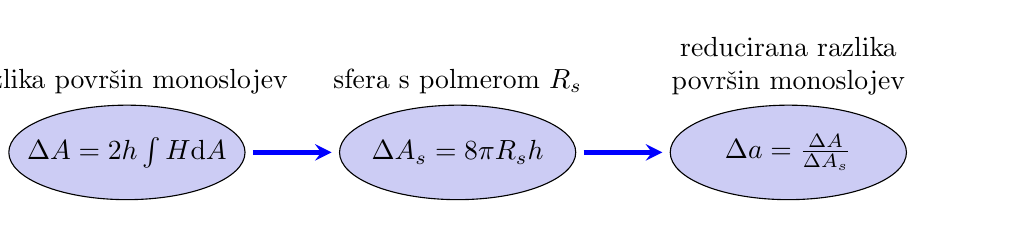
\begin{tikzpicture}
   		\hspace{-0.9cm}
   		\definecolor{FillColor1}{RGB}{0,0,200, 255};
   		\def \ELen {1.5};
   		\def \EHight {0.6};
   		\def \Gap {0.1};
   		\def \ALen {1.0};
   		\def \textGap {0.9}
   		
   		\draw [fill=FillColor1, fill opacity=0.2] (0,0) ellipse ({\ELen} and {\EHight}) node[anchor=center, black, opacity=1.0] {$\Delta A=2h\int H \dif{A}$};
   		
   		\node[black](textdA) at (0cm, {\textGap}){razlika površin monoslojev};
   		
   		\draw [blue, ->,  -stealth , ultra thick   ] (\ELen+\Gap , 0) -- (\ELen+\Gap+\ALen,0) ;
   		
   		\draw [fill=FillColor1, fill opacity=0.2] (2*\ELen+2*\Gap+\ALen,0) ellipse ({\ELen} and {\EHight}) node[anchor=center, black, opacity=1.0] {$\Delta A_s=8\pi R_s h$};
   		
   		\node[black](textdA) at (2*\ELen+2*\Gap+\ALen, {\textGap}){sfera s polmerom $R_s$};
   		
   		\draw [blue, ->,  -stealth , ultra thick   ] (3*\ELen+3*\Gap+\ALen , 0) -- (3*\ELen+3*\Gap+2*\ALen , 0) ;
   		
   		\draw [fill=FillColor1, fill opacity=0.2] (4*\ELen+4*\Gap+2*\ALen,0) ellipse ({\ELen} and {\EHight}) node[anchor=center, black, opacity=1.0] {$\Delta a=\frac{\Delta A}{\Delta A_s}$};
   		
   		\node[black, align=center](textdA) at (4*\ELen+4*\Gap+2*\ALen, {\textGap+0.2}){reducirana razlika\\površin monoslojev};
   		
   		\end{tikzpicture}
   	\end{frame}
   	
   	\begin{frame}
   		\frametitle{Fazni diagrami brez medmembranske interakcije}
   		\begin{tikzpicture}[remember picture,overlay]
   		\def \xfromcenter  {3.8}
   		\def \yfromcenter {0.5}
   		
   		\node (slika1) at ($(current page.center)+ (-\xfromcenter,\yfromcenter cm)$)
   		{\includegraphics[width=.3\textwidth]{{minimizacija_q1_0_q2_0_da0_0_R_0.5_eta_0.98_sirinav_0.01_sirinada_0.05}.pdf}};
   		
   		\node[anchor=north] at ($(current page.center) + (-0.97*\xfromcenter, \yfromcenter + 2)$) {\tiny$R=0.5,  q=0, \gamma=0, \eta=0.98 $};
   		
   		\node[] (legenda) at ($(current page.center) + (0, \yfromcenter)$)
   		{\includegraphics[width=.33\textwidth]{legenda.pdf}} node[align=center, xshift=4.5cm] at (Vograditev) {};
   		
   		\node (slika2) at ($(current page.center) + (\xfromcenter, \yfromcenter)$)
   		{\includegraphics[width=.3\textwidth]{{minimizacija_q1_10*Pi_q2_0_da0_0_R_0.5_eta_0.98_sirinav_0.01_sirinada_0.05}.pdf}};
   		
   		\node[anchor=north] at ($(current page.center) + (1.03*\xfromcenter, \yfromcenter + 2)$) {\tiny$R=0.5,  q=10\pi, \gamma=0, \eta=0.98 $};
   		
   		
   		{
   			\setlength{\fboxrule}{0pt}%
   			\node[] (itemize1) [below=0cm and 0cm of slika1, xshift=1cm] {\framebox{\normalsize
   					{\begin{varwidth}{0.55\linewidth}
   						\begin{itemize}
   						\item $q=0$: fazni diagram ni odvisen od $\Delta a_0$
   						\item U rob $\rightarrow$ vesikel s popolnimi prečnimi stenami v območju vesikla z nepopolnimi prečnimi stenami
   						\end{itemize}
   						\end{varwidth}
   					}
   				}};
   			}
   			
   			{
   				\setlength{\fboxrule}{0pt}%
   				\node (itemize1) [below=0cm of slika2, xshift=-0.4cm] {\framebox{\normalsize
   						{\begin{varwidth}{0.55\linewidth}
   							\begin{itemize}
   							\item stabilizirani vesikli z nepopolnimi prečnimi stenami, tubuli in vzdlžno steno v primerjavi z vesikli s popolnimi prečnimi stenami
   							\end{itemize}
   							\end{varwidth}
   						}
   					}};
   				}
   				
   				\end{tikzpicture}
   			\end{frame}
   	  
\end{document}